\section{Random Forests}

\begin{frame}{From Decision Trees to Ensembles}
\begin{columns}[T]
\column{0.52\textwidth}
\begin{itemize}
  \item A single deep decision tree overfits.
  \pause
  \item Recall: training accuracy increases with depth, but validation accuracy plateaus or drops.
  \pause
  \item The fix: train many different trees and combine their predictions.
  \pause
  \item Averaging reduces variance.
\end{itemize}

\pause
\column{0.48\textwidth}
\centering
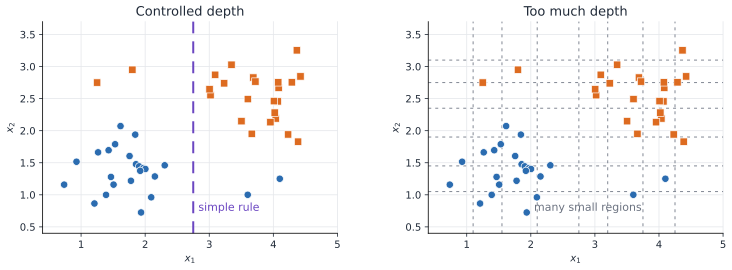
\includegraphics[width=\textwidth]{figures/decision_trees/decision_tree_overfitting.pdf}
\end{columns}
\end{frame}

\begin{frame}{Why Random Forests?}
\begin{columns}[T]
\column{0.52\textwidth}
\begin{itemize}
  \item A single tree is a high-variance estimator.
  \pause
  \item Small changes in training data lead to very different trees.
  \pause
  \item If we train many trees on different data and average, variance drops.
  \pause
  \item But to make trees different, we need different training sets.
\end{itemize}

\pause
\column{0.48\textwidth}
\begin{rlintuition}
Averaging many noisy but independent predictions is more stable than one perfect prediction.
\end{rlintuition}
\end{columns}
\end{frame}

\begin{frame}{Bagging: Bootstrap Sampling}
\begin{columns}[T]
\column{0.53\textwidth}
\begin{itemize}
  \item Start with dataset $D$ of size $n$.
  \pause
  \item For $b=1,\dots,B$, draw a bootstrap sample:
  \begin{equation}
    D^{(b)} \sim \text{Resample}(D,\,n)\text{ with replacement}.
    \label{eq:bootstrap-sample}
  \end{equation}
  \pause
  \item Each $D^{(b)}$ has size $n$ but many examples appear multiple times.
  \pause
  \item About $63\%$ of the original $n$ examples appear in each sample.
\end{itemize}

\pause
\column{0.47\textwidth}
\centering
\includegraphics[width=\textwidth]{figures/random_forests/bagging_diagram.pdf}
\end{columns}
\end{frame}

\begin{frame}{Training a Forest}
\begin{itemize}
  \item For each bootstrap sample $D^{(b)}$, train one full decision tree $T_b$.
  \pause
  \item Each tree is trained independently.
  \pause
  \item Use the same impurity criterion and stopping rules as before.
  \pause
  \item Grow trees to completion (or use a fixed max depth).
  \pause
  \item After training, you have $B$ trees.
\end{itemize}
\end{frame}

\begin{frame}{Feature Subsampling at Each Node}
\begin{columns}[T]
\column{0.53\textwidth}
\begin{itemize}
  \item When searching for the best split at a node, do not consider all $d$ features.
  \pause
  \item Instead, randomly select $m$ features.
  \pause
  \item Search for the best split using only those $m$ features.
  \pause
  \item Common choices:
  \begin{itemize}
    \item Classification: $m = \lfloor\sqrt{d}\rfloor$
    \item Regression: $m = \lfloor d/3 \rfloor$
  \end{itemize}
\end{itemize}

\pause
\column{0.47\textwidth}
\centering
\includegraphics[width=\textwidth]{figures/random_forests/feature_subsampling.pdf}
\end{columns}
\end{frame}

\begin{frame}{Why Feature Subsampling?}
\begin{itemize}
  \item Without it, all trees pick the same dominant feature at the root.
  \pause
  \item All trees then split the same way, and their predictions are highly correlated.
  \pause
  \item Averaging correlated predictions does not reduce variance much.
  \pause
  \item Feature subsampling forces trees to explore different features.
  \pause
  \item Decorrelated trees reduce variance more effectively.
\end{itemize}
\end{frame}

\begin{frame}{Forest Prediction (Classification)}
\begin{columns}[T]
\column{0.53\textwidth}
\begin{itemize}
  \item Each tree $T_b$ makes a prediction $\hat{y}^{(b)}(x)$ for a new example $x$.
  \pause
  \item The forest prediction is the majority vote:
  \begin{equation}
    \hat{y}(x) = \text{majority}\bigl\{\hat{y}^{(1)}(x),\,\dots,\,\hat{y}^{(B)}(x)\bigr\}.
    \label{eq:forest-vote}
  \end{equation}
  \pause
  \item In case of a tie, the class with the most votes wins.
\end{itemize}

\pause
\column{0.47\textwidth}
\centering
\includegraphics[width=\textwidth]{figures/random_forests/forest_vote.pdf}
\end{columns}
\end{frame}

\begin{frame}{Forest Prediction (Regression)}
\begin{itemize}
  \item For regression, each tree $T_b$ predicts a continuous value $\hat{y}^{(b)}(x)$.
  \pause
  \item The forest prediction is the mean:
  \begin{equation}
    \hat{y}(x) = \frac{1}{B}\sum_{b=1}^{B}\hat{y}^{(b)}(x).
    \label{eq:forest-mean}
  \end{equation}
  \pause
  \item Averaging many estimates reduces variance.
\end{itemize}
\end{frame}

\begin{frame}{Worked Numerical Example}
\small
\begin{itemize}
  \item Five trees make the following predictions on one example:
  \[
    \hat{y}^{(1)} = A,\quad
    \hat{y}^{(2)} = A,\quad
    \hat{y}^{(3)} = B,\quad
    \hat{y}^{(4)} = A,\quad
    \hat{y}^{(5)} = B.
  \]
  \pause
  \item Class counts: $A$ appears 3 times, $B$ appears 2 times.
  \pause
  \item The forest prediction is $\hat{y} = A$ (majority class).
  \pause
  \item Even if one tree is wrong, the forest is robust.
\end{itemize}
\end{frame}

\begin{frame}{Out-of-Bag Error}
\begin{columns}[T]
\column{0.53\textwidth}
\begin{itemize}
  \item When we draw a bootstrap sample of size $n$, about 37\% of the original examples are left out.
  \pause
  \item These ``out-of-bag'' (OOB) samples are not used to train that tree.
  \pause
  \item Use the OOB samples as a free validation set.
  \pause
  \item The OOB error is a good estimate of test error.
\end{itemize}

\pause
\column{0.47\textwidth}
\centering
\includegraphics[width=\textwidth]{figures/random_forests/oob_illustration.pdf}
\end{columns}
\end{frame}

\begin{frame}{Variance Reduction}
\begin{itemize}
  \item If $B$ trees were independent, averaging would reduce variance by a factor of $1/B$.
  \pause
  \item In practice, trees are correlated because they grow from similar data.
  \pause
  \item Feature subsampling reduces this correlation.
  \pause
  \item Error typically decreases quickly at first, then plateaus.
  \pause
  \item More trees reduce variance, but do not cause overfitting.
\end{itemize}
\end{frame}

\begin{frame}{Feature Importance}
\begin{itemize}
  \item Which features are most useful for prediction?
  \pause
  \item Compute the mean impurity decrease for each feature across all trees.
  \pause
  \item For feature $j$, sum the impurity decrease $\Delta I$ over all nodes in all trees where $j$ was chosen as the split feature:
  \begin{equation}
    \text{FI}(j) = \frac{1}{B}\sum_{b=1}^{B}\sum_{\substack{\text{nodes in }T_b \\ \text{split on }j}} \frac{n_m}{n}\,\Delta I.
    \label{eq:feature-importance}
  \end{equation}
  \pause
  \item Normalize so importances sum to 1.
  \pause
  \item High importance means the feature is used in many high-impact splits.
\end{itemize}
\end{frame}

\begin{frame}{Decision Boundary Comparison}
\centering
\includegraphics[width=0.92\textwidth]{figures/random_forests/boundary_comparison.pdf}

\vspace{0.35em}
\begin{itemize}
  \item Left: single decision tree (jagged, many small regions).
  \pause
  \item Right: random forest (smoother, more stable regions).
\end{itemize}
\end{frame}

\begin{frame}{Error vs Number of Trees}
\centering
\includegraphics[width=0.92\textwidth]{figures/random_forests/error_vs_trees.pdf}

\vspace{0.35em}
\begin{itemize}
  \item OOB error and test error decrease with $B$.
  \pause
  \item Curve flattens after a certain point.
  \pause
  \item More trees do not cause overfitting.
\end{itemize}
\end{frame}

\begin{frame}{Random Forests vs Single Decision Tree}
\begin{columns}[T]
\column{0.5\textwidth}
\textbf{Single Tree}
\begin{itemize}
  \item Fast to train and predict.
  \pause
  \item Easy to interpret.
  \pause
  \item High variance, overfits easily.
  \pause
  \item Better on clean, small data.
\end{itemize}

\pause
\column{0.5\textwidth}
\textbf{Random Forest}
\begin{itemize}
  \item Slower to train and predict.
  \pause
  \item Hard to interpret.
  \pause
  \item Low variance, generalizes well.
  \pause
  \item Better on messy, large data.
\end{itemize}
\end{columns}
\end{frame}

\begin{frame}{Key Hyperparameters}
\begin{itemize}
  \item \textbf{\texttt{n\_estimators}} $B$: number of trees. More is better (no overfitting), but slower.
  \pause
  \item \textbf{\texttt{max\_features}} $m$: number of features to sample at each split. Smaller $m$ reduces correlation but may miss good splits.
  \pause
  \item \textbf{\texttt{max\_depth}}: max depth of each tree. Can limit to control per-tree complexity.
  \pause
  \item \textbf{\texttt{min\_samples\_leaf}}: min samples at a leaf. Prevents very small leaves.
\end{itemize}
\end{frame}

\begin{frame}{When RF Works and When It Fails}
\begin{columns}[T]
\column{0.5\textwidth}
\textbf{Works well when}
\begin{itemize}
  \item data is tabular,
  \pause
  \item many features,
  \pause
  \item moderate to large $n$,
  \pause
  \item noisy labels.
\end{itemize}

\pause
\column{0.5\textwidth}
\textbf{Can fail when}
\begin{itemize}
  \item need a single interpretable rule,
  \pause
  \item sparse high-dimensional text,
  \pause
  \item very small data,
  \pause
  \item rare classes dominate.
\end{itemize}
\end{columns}
\end{frame}

\begin{frame}{Summary}
\begin{itemize}
  \item Random forests train multiple trees on bootstrap samples.
  \item Feature subsampling decorrelates trees and improves variance reduction.
  \item Classification uses majority vote; regression uses the mean.
  \item Out-of-bag error provides a free validation estimate.
  \item More trees reduce variance without overfitting.
  \item Feature importance ranks useful features by impurity decrease.
\end{itemize}
\end{frame}

\begin{frame}{Lab Connection}
\begin{itemize}
  \item Implement the bagging loop: bootstrap sampling and independent tree training.
  \pause
  \item Add feature subsampling to the tree split search.
  \pause
  \item Implement majority vote and mean predictions.
  \pause
  \item Compare single tree vs forest on tabular data (Iris).
  \pause
  \item Report OOB error and compare with test accuracy.
  \pause
  \item Extract and visualize feature importances.
\end{itemize}
\end{frame}
